\documentclass[12pt,a4paper]{report}

% ---------------------------------------------------------------------------
% Préambule
% ---------------------------------------------------------------------------
\usepackage[numbers,sort&compress]{natbib}
\usepackage[french]{babel}
\usepackage[utf8]{inputenc}
\usepackage[T1]{fontenc}
\usepackage{lmodern}
\usepackage{microtype}
\usepackage[margin=2.5cm,headheight=14pt]{geometry}
\usepackage{graphicx}
\usepackage{booktabs}
\usepackage{array}
\usepackage{multirow}
\usepackage{longtable}
\usepackage{amsmath}
\usepackage{setspace}
\usepackage{titlesec}
\usepackage{fancyhdr}
\usepackage{caption}
\usepackage{listings}
\usepackage{xcolor}
\usepackage[hidelinks]{hyperref}
\usepackage{xurl}

\onehalfspacing
\emergencystretch=3em

\lstset{
  basicstyle=\ttfamily\footnotesize,
  breaklines=true,
  frame=single,
  columns=fullflexible,
  showstringspaces=false,
  captionpos=b,
}

\pagestyle{fancy}
\fancyhf{}
\fancyhead[L]{\small Estimation de la valeur des biens immobiliers résidentiels au Sénégal}
\fancyhead[R]{\small\thepage}
\renewcommand{\headrulewidth}{0.4pt}

\titleformat{\chapter}[display]
  {\normalfont\huge\bfseries}{\chaptertitlename\ \thechapter}{20pt}{\Huge}
\titlespacing*{\chapter}{0pt}{0pt}{40pt}

% ---------------------------------------------------------------------------
% Informations du document, à adapter si besoin
% ---------------------------------------------------------------------------
\newcommand{\auteurUn}{[Votre Nom Complet]}
\newcommand{\sujetTitre}{Estimation de la valeur des biens immobiliers résidentiels au Sénégal : prédiction des prix, optimisation des paramètres d'entraînement et interface graphique interactive}
\newcommand{\anneeAcademique}{2025-2026}

\begin{document}

% ---------------------------------------------------------------------------
% Page de garde
% ---------------------------------------------------------------------------
\begin{titlepage}
\begin{center}

{\Large\bfseries Dakar Institute of Technology}\\[0.3cm]

\vspace{0.3cm}

\includegraphics[width=0.45\textwidth]{figures/logo_dit.png}\\[0.5cm]

{\small Habilitation n\textsuperscript{o}3386-21 FEV.2024}\\[0.6cm]

{\small \textbf{Domaine :} Sciences et Technologies}\\
{\small \textbf{Département :} Informatique}\\
{\small \textbf{Spécialité :} Intelligence Artificielle}\\[1cm]

{\Large\bfseries Projet Informatique}\\[1cm]

{\small Présenté par :}\\[0.3cm]
{\large \auteurUn}\\[1.5cm]

\rule{0.8\textwidth}{0.4pt}\\[0.4cm]
{\Large\bfseries SUJET :}\\[0.4cm]
{\Large \sujetTitre}\\[0.4cm]
\rule{0.8\textwidth}{0.4pt}\\[2cm]

{\small Soutenu le : 27/08/2026}\\[0.3cm]
{\small \textbf{Année Académique :} \anneeAcademique}

\vfill
\end{center}
\end{titlepage}


% ---------------------------------------------------------------------------
% Front matter
% ---------------------------------------------------------------------------
\pagenumbering{roman}

\chapter*{Dédicace}
\addcontentsline{toc}{chapter}{Dédicace}

% À adapter librement, texte de départ à personnaliser.
À ma famille, pour son soutien indéfectible tout au long de ce projet.

\chapter*{Remerciements}
\addcontentsline{toc}{chapter}{Remerciements}

% À adapter librement, texte de départ à personnaliser.
Je tiens à remercier l'ensemble du corps enseignant du Dakar Institute of Technology pour
l'encadrement apporté tout au long de ce projet informatique, ainsi que toute personne ayant
contribué, de près ou de loin, à sa réalisation.

\chapter*{Glossaire}
\addcontentsline{toc}{chapter}{Glossaire}

\begin{description}
  \item[FCFA] Franc de la Communauté Financière Africaine, monnaie utilisée au Sénégal.
  \item[Modèle hédonique] Modèle économétrique postulant que le prix d'un bien composite (ex. un logement) se décompose en la somme des valeurs implicites de ses caractéristiques (surface, localisation, etc.).
  \item[RMSE] \emph{Root Mean Squared Error} : racine de l'erreur quadratique moyenne, métrique d'évaluation pénalisant fortement les grandes erreurs.
  \item[MAE] \emph{Mean Absolute Error} : erreur absolue moyenne entre les valeurs prédites et réelles.
  \item[MAPE] \emph{Mean Absolute Percentage Error} : erreur moyenne exprimée en pourcentage de la valeur réelle.
  \item[$R^2$] Coefficient de détermination : part de la variance de la variable cible expliquée par le modèle.
  \item[Random Forest] Algorithme d'apprentissage ensembliste combinant un grand nombre d'arbres de décision entraînés sur des sous-échantillons aléatoires des données.
  \item[XGBoost] \emph{Extreme Gradient Boosting} : algorithme de boosting de gradient optimisé, construisant les arbres de façon séquentielle pour corriger les erreurs des précédents.
  \item[MLP] \emph{Multi-Layer Perceptron} : réseau de neurones artificiels à propagation avant, composé d'une ou plusieurs couches cachées.
  \item[Hyperparamètre] Paramètre de configuration d'un modèle fixé avant l'entraînement (ex. profondeur d'un arbre, taux d'apprentissage), par opposition aux paramètres appris à partir des données.
  \item[One-Hot Encoding] Technique d'encodage transformant une variable catégorielle en un ensemble de variables binaires indicatrices.
  \item[Web scraping] Technique de collecte automatisée de données publiées sur des pages web.
\end{description}


\renewcommand{\listfigurename}{Liste des figures}
\listoffigures
\clearpage

\renewcommand{\listtablename}{Liste des tableaux}
\listoftables
\clearpage

\chapter*{Résumé}
\addcontentsline{toc}{chapter}{Résumé}

Ce projet informatique de Master 1 présente le développement d'un système d'estimation
automatique de la valeur des biens immobiliers résidentiels (maisons et appartements) au
Sénégal, à partir de techniques d'apprentissage automatique. L'objectif est double : d'une
part comparer plusieurs modèles de prédiction en optimisant systématiquement leurs
hyperparamètres, et d'autre part rendre ces résultats accessibles à travers une interface
graphique interactive.

En l'absence de jeu de données immobilier sénégalais existant, un corpus de 660 annonces de
vente a été collecté par extraction automatisée (\emph{web scraping}) depuis la plateforme
Expat-Dakar, couvrant l'ensemble du territoire national. Après nettoyage (suppression des prix
non exploitables et des biens hors périmètre résidentiel unitaire), un jeu de données de 603
annonces a été retenu, décrit par la surface, le nombre de chambres, le type de bien et le
quartier.

Quatre modèles ont été entraînés et comparés : une régression linéaire (référence), une
forêt aléatoire (\emph{Random Forest}), un modèle de \emph{gradient boosting} (XGBoost), et un
réseau de neurones multicouches (MLP) — les trois derniers optimisés par recherche
aléatoire d'hyperparamètres avec validation croisée. Le modèle Random Forest optimisé obtient
les meilleures performances sur le jeu de test (MAE de 73,3 millions FCFA, MAPE de 34,0~\%,
$R^2$ de 0,751), devançant XGBoost et le réseau de neurones — un résultat cohérent avec la
littérature sur des jeux de données tabulaires de taille modeste.

Une application interactive développée avec Streamlit permet enfin d'estimer le prix d'un bien
à partir de ses caractéristiques, d'explorer le jeu de données et de comparer visuellement les
performances des différents modèles.

\vspace{0.5cm}
\noindent\textbf{Mots-clés :} immobilier, apprentissage automatique, optimisation
d'hyperparamètres, Random Forest, XGBoost, réseau de neurones, Sénégal, Streamlit.

\chapter*{Abstract}
\addcontentsline{toc}{chapter}{Abstract}

This Master 1 computer science project presents the development of an automatic valuation
system for residential real estate (houses and apartments) in Senegal, based on machine
learning techniques. The goal is twofold: to compare several prediction models through
systematic hyperparameter optimization, and to make the results accessible through an
interactive graphical interface.

In the absence of any existing Senegalese real-estate dataset, a corpus of 660 sale listings
was collected through automated web scraping from the Expat-Dakar platform, covering the
whole country. After cleaning (removal of non-exploitable prices and of properties outside the
single-unit residential scope), a dataset of 603 listings was retained, described by surface
area, number of bedrooms, property type, and neighborhood.

Four models were trained and compared: a linear regression (baseline), a Random Forest, a
gradient boosting model (XGBoost), and a multi-layer perceptron (MLP) neural network — the
latter three tuned through randomized hyperparameter search with cross-validation. The
optimized Random Forest achieved the best performance on the test set (MAE of 73.3 million
FCFA, MAPE of 34.0\%, $R^2$ of 0.751), outperforming both XGBoost and the neural network — a
result consistent with the literature on modestly sized tabular datasets.

An interactive web application built with Streamlit allows users to estimate a property's
price from its characteristics, explore the dataset, and visually compare model performance.

\vspace{0.5cm}
\noindent\textbf{Keywords:} real estate, machine learning, hyperparameter optimization, Random
Forest, XGBoost, neural network, Senegal, Streamlit.


\chapter*{Sommaire}
\addcontentsline{toc}{chapter}{Sommaire}
\begin{enumerate}
  \item[] Introduction
  \item[] Chapitre I : État de l'art
  \item[] Chapitre II : Analyse de besoins et méthodologie
  \item[] Chapitre III : Implémentation
  \item[] Conclusion générale
  \item[] Bibliographie et webographie
  \item[] Annexes
\end{enumerate}
\clearpage

% ---------------------------------------------------------------------------
% Corps du document
% ---------------------------------------------------------------------------
\pagenumbering{arabic}

\chapter{Introduction}

\section{Contexte et justification}

Le secteur immobilier occupe une place croissante dans l'économie sénégalaise, porté par
l'urbanisation rapide de l'agglomération dakaroise et le développement de pôles urbains
secondaires (Diamniadio, Thiès, Mbour). Pourtant, contrairement à des marchés plus matures où
des bases de données de transactions publiques (cadastre ouvert, historiques notariaux)
permettent une estimation relativement transparente des prix, le marché sénégalais souffre
d'un déficit important d'information centralisée : les prix affichés sur les plateformes
d'annonces sont négociables, très hétérogènes d'un quartier à l'autre, et aucune base de
données publique ne permet aujourd'hui d'objectiver la valeur d'un bien à partir de ses
caractéristiques.

Cette opacité pénalise autant les particuliers (acheteurs, vendeurs) que les professionnels
(agences immobilières, banques accordant des prêts hypothécaires) qui doivent s'appuyer sur
l'expertise de terrain ou sur la méthode dite « des comparables », intrinsèquement subjective
et chronophage. L'essor de l'apprentissage automatique (\emph{machine learning}) et la
multiplication des données disponibles en ligne (notamment via les plateformes d'annonces
immobilières) ouvrent la voie à des modèles d'estimation automatique de la valeur des biens,
communément appelés \emph{Automated Valuation Models} (AVM) dans la littérature.

C'est dans ce contexte que s'inscrit ce projet informatique : construire, à partir de données
réellement observées sur le marché sénégalais, un modèle capable d'estimer le prix d'un bien
résidentiel (maison ou appartement), tout en explorant systématiquement l'apport de
l'optimisation des hyperparamètres d'entraînement sur la qualité des prédictions, et en rendant
ce modèle accessible via une interface graphique interactive plutôt que réservé à un usage
technique.

\section{Objectifs de la recherche}

Ce projet poursuit trois objectifs principaux :

\begin{enumerate}
  \item \textbf{Constituer un jeu de données exploitable} sur les prix des biens immobiliers
  résidentiels au Sénégal, en l'absence de source publique existante, par collecte automatisée
  de données d'annonces réelles.
  \item \textbf{Comparer plusieurs familles de modèles} de prédiction du prix (régression
  linéaire, méthodes ensemblistes à base d'arbres, réseau de neurones), en optimisant
  systématiquement leurs hyperparamètres d'entraînement par recherche aléatoire avec validation
  croisée, afin d'identifier l'approche la plus pertinente au regard du volume de données
  disponible.
  \item \textbf{Développer une interface graphique interactive} permettant à un utilisateur non
  technique d'obtenir une estimation de prix à partir des caractéristiques d'un bien, et
  d'explorer visuellement les données et les performances des modèles.
\end{enumerate}

\section{Structure du projet informatique}

Ce document est organisé en trois chapitres. Le \textbf{Chapitre~I} dresse un état de l'art du
domaine, à la fois sur les méthodes classiques d'évaluation immobilière et sur les travaux de
recherche appliquant l'apprentissage automatique à ce problème, en identifiant les zones encore
peu explorées, en particulier dans le contexte ouest-africain. Le \textbf{Chapitre~II} détaille
l'analyse des besoins, les sources de données mobilisées, le processus de collecte et de
pré-traitement, ainsi que la méthodologie de modélisation et d'évaluation retenue. Le
\textbf{Chapitre~III} présente l'implémentation réalisée : l'analyse exploratoire des données,
les résultats obtenus pour chaque modèle, leur interprétation et leur mise en perspective avec
la littérature, ainsi que les outils et l'architecture de la solution développée, incluant
l'interface graphique interactive. Une conclusion générale dresse le bilan du projet et propose
des perspectives d'amélioration.

\section{Conclusion}

Ce chapitre introductif a situé le projet dans son contexte : un marché immobilier sénégalais
en expansion mais peu documenté, pour lequel les techniques d'apprentissage automatique offrent
une opportunité concrète d'objectiver l'estimation des prix. Les trois objectifs retenus
(collecte de données, modélisation optimisée, restitution interactive) structurent l'ensemble
de la démarche présentée dans les chapitres suivants.

\chapter{État de l'art}

\section{État de l'art sur le domaine d'application}

L'estimation de la valeur d'un bien immobilier repose historiquement sur le \textbf{modèle
hédonique}, formalisé par \citet{rosen1974hedonic}. Ce modèle postule qu'un bien composite
comme un logement peut être décomposé en un ensemble de caractéristiques (surface, nombre de
pièces, localisation, qualité de construction, etc.), chacune contribuant implicitement au prix
final observé sur le marché. Cette approche, traditionnellement opérationnalisée par une
régression linéaire multiple, reste la référence en économie urbaine et sous-tend encore la
méthode dite « des comparables » utilisée par les agents immobiliers et notaires : le prix d'un
bien est estimé par analogie avec des transactions récentes de biens aux caractéristiques
proches.

Cette approche présente cependant des limites bien documentées : elle suppose des relations
linéaires entre caractéristiques et prix, peine à capturer les interactions complexes entre
variables (par exemple, l'effet de la surface sur le prix n'est pas le même selon le quartier),
et dépend fortement de la disponibilité de transactions comparables récentes, une condition
difficile à remplir dans un marché comme celui du Sénégal, où les données de transactions ne
sont pas centralisées.

L'essor de l'apprentissage automatique a permis l'émergence des \emph{Automated Valuation
Models} (AVM), qui remplacent ou complètent le modèle hédonique classique par des algorithmes
capables de capturer des relations non linéaires et des interactions complexes entre
caractéristiques, sans hypothèse a priori sur la forme fonctionnelle de la relation entre les
variables explicatives et le prix.

\section{État de l'art sur les travaux de recherche pertinents liés au sujet}

Plusieurs familles de modèles ont été appliquées à la prédiction de prix immobiliers dans la
littérature récente.

Les \textbf{méthodes ensemblistes à base d'arbres de décision} occupent une place centrale.
\citet{breiman2001randomforests} a introduit le \emph{Random Forest}, qui combine un grand
nombre d'arbres entraînés sur des sous-échantillons aléatoires des données et des variables,
réduisant la variance par rapport à un arbre unique. \citet{chen2016xgboost} a ensuite proposé
XGBoost, une implémentation optimisée du \emph{gradient boosting}, qui construit les arbres de
façon séquentielle pour corriger les erreurs des précédents. Appliqués à la prédiction de prix
immobiliers, \citet{truong2020housing} comparent régression linéaire, k plus proches voisins,
CART et méthodes ensemblistes, et montrent la supériorité systématique des approches
ensemblistes sur les modèles linéaires classiques. \citet{sharma2024optimal} comparent plus
spécifiquement régression linéaire multiple, SVR, Random Forest, MLP et XGBoost sur le jeu de
données Ames Housing (Iowa, États-Unis) et concluent à la supériorité de XGBoost, avec un
$R^2$ proche de 0,89, un résultat obtenu toutefois sur un jeu de données nettement plus riche
(79 variables descriptives) que celui mobilisé dans ce projet.

Les \textbf{réseaux de neurones profonds} ont également été explorés. \citet{yazdani2021mldl}
comparent modèles hédoniques classiques, méthodes de machine learning (Random Forest, k plus
proches voisins) et de deep learning pour la prédiction de prix immobiliers, et observent que
l'avantage des réseaux de neurones dépend fortement du volume de données disponible : sur des
jeux de données de taille modeste, les méthodes ensemblistes à base d'arbres restent souvent
compétitives, voire supérieures, aux architectures de deep learning.

Enfin, un travail directement pertinent pour le contexte de ce projet est celui de
\citet{nwankwo2023lagos}, qui appliquent plusieurs modèles de machine learning (dont un réseau
de neurones artificiel et XGBoost) à la prédiction des prix immobiliers à Lagos, au Nigeria, un
marché ouest-africain partageant avec le Sénégal des caractéristiques structurelles proches
(données peu centralisées, forte hétérogénéité des annonces en ligne). Les auteurs confirment
l'efficacité des approches ensemblistes et des réseaux de neurones dans ce contexte, tout en
soulignant le rôle déterminant des variables de localisation.

L'écosystème logiciel de ce projet s'appuie par ailleurs sur la bibliothèque scikit-learn
\citep{pedregosa2011scikitlearn}, largement utilisée dans la littérature pour l'implémentation
reproductible de pipelines de machine learning.

\section{Identification des zones de recherche manquantes liées au sujet}

Cette revue de la littérature met en évidence plusieurs zones encore peu explorées, que ce
projet cherche en partie à adresser :

\begin{itemize}
  \item \textbf{Absence de données et de travaux spécifiques au Sénégal.} Contrairement au
  Nigeria \citep{nwankwo2023lagos} ou aux marchés occidentaux disposant de jeux de données de
  référence (Ames Housing, Boston Housing), aucun jeu de données immobilier sénégalais n'est
  publiquement disponible, et aucun travail de recherche appliquant le machine learning à ce
  marché n'a été identifié au moment de la rédaction de ce document.
  \item \textbf{Comparaison systématique méthodes ensemblistes / deep learning sur données
  ouest-africaines restreintes.} La littérature suggère que l'avantage du deep learning sur les
  méthodes ensemblistes dépend du volume de données \citep{yazdani2021mldl}, mais ce compromis
  n'a pas été quantifié sur un marché immobilier africain à faible volume de données
  structurées.
  \item \textbf{Accessibilité des outils produits.} La grande majorité des travaux cités se
  limitent à une évaluation académique des modèles, sans restitution accessible à un utilisateur
  non technique, un manque que ce projet adresse via le développement d'une interface graphique
  interactive.
\end{itemize}

\section{Conclusion}

Le modèle hédonique reste le cadre théorique de référence pour l'estimation immobilière, mais
les approches d'apprentissage automatique, en particulier les méthodes ensemblistes à base
d'arbres, s'imposent progressivement comme des alternatives plus performantes, sous réserve
d'un volume de données suffisant. Le contexte sénégalais, marqué par l'absence de données
publiques structurées, constitue à la fois la principale difficulté méthodologique de ce projet
et sa principale zone de contribution : la constitution d'un premier jeu de données exploitable
et la comparaison empirique de plusieurs familles de modèles sur ce marché spécifique.

\chapter{Analyse de besoins et méthodologie}

\section{I. Spécification des besoins et des données}

\subsection{Analyse et spécification des besoins}

Les utilisateurs finaux visés par ce projet sont les particuliers souhaitant estimer la valeur
d'un bien avant une transaction, ainsi que les professionnels (agences immobilières) souhaitant
disposer d'un outil d'aide à la décision rapide.

\textbf{Besoins fonctionnels :}
\begin{itemize}
  \item Estimer le prix d'un bien résidentiel (maison ou appartement) à partir de ses
  caractéristiques principales (type, quartier, surface, nombre de chambres).
  \item Comparer les résultats de plusieurs modèles pour un même bien.
  \item Explorer visuellement le jeu de données ayant servi à l'entraînement (distribution des
  prix, prix par quartier, etc.).
  \item Visualiser les performances comparées des modèles.
\end{itemize}

\textbf{Besoins non fonctionnels :}
\begin{itemize}
  \item Accessibilité via une interface web, sans compétence technique requise.
  \item Reproductibilité du pipeline de collecte, nettoyage et entraînement.
  \item Transparence sur la marge d'erreur des estimations produites.
\end{itemize}

\subsection{Sources de données}

Une recherche préalable a permis d'écarter plusieurs pistes de données existantes :
\begin{itemize}
  \item aucun jeu de données immobilier sénégalais n'est disponible sur les plateformes usuelles
  (Kaggle) ;
  \item l'Agence Nationale de la Statistique et de la Démographie (ANSD) publie des indices
  macro-économiques du secteur (indice du coût de la construction, indice des prix des
  matériaux), mais aucune donnée au niveau transaction ;
  \item aucun portail cadastral ouvert, comparable à celui existant en France, n'est disponible
  pour le Sénégal.
\end{itemize}

Faute de source structurée existante, les données ont été collectées par extraction
automatisée (\emph{web scraping}) depuis \textbf{Expat-Dakar}
(\url{https://www.expat-dakar.com/}), plateforme d'annonces généralistes hébergeant plusieurs
milliers d'annonces immobilières actives. Ce choix a été validé par une double vérification :
la structure des pages (attributs \texttt{data-t-listing\_*} intégrés directement dans le HTML,
encodant prix, type de bien, localisation et identifiant de façon structurée) permet une
extraction fiable, et le fichier \texttt{robots.txt} du site autorise l'accès aux pages
d'annonces (seuls les répertoires \texttt{/admin/}, \texttt{/compte/} et \texttt{/cdn-cgi/} sont
exclus).

\subsection{Processus de collecte}

La collecte a été réalisée avec un script Python (\texttt{src/scraper.py}) s'appuyant sur les
bibliothèques \texttt{requests} et \texttt{BeautifulSoup}. Le périmètre retenu couvre :
\begin{itemize}
  \item les annonces de \textbf{vente} (à l'exclusion de la location, pour ne pas mélanger deux
  marchés aux dynamiques de prix différentes) ;
  \item les catégories \textbf{maisons à vendre} et \textbf{appartements à vendre} (à
  l'exclusion des terrains nus et des biens commerciaux, hors périmètre résidentiel) ;
  \item l'ensemble du territoire sénégalais (pas de restriction géographique a priori).
\end{itemize}

Pour chaque annonce, les champs suivants sont extraits : identifiant, titre, catégorie, prix
(FCFA), quartier, ville/région, nombre de chambres, surface (m\textsuperscript{2}), date de
publication et URL. La pagination est parcourue jusqu'à réception d'une page vide ou d'une
réponse HTTP 404 signalant la fin des résultats, avec un délai d'une seconde et demie entre
chaque requête afin de limiter la charge sur le serveur cible. La collecte a produit
\textbf{660 annonces brutes} (330 maisons, 330 appartements), sans doublon.

\subsection{Pré-processing des données}

Le nettoyage du jeu de données brut (détaillé et exécuté dans le notebook
\texttt{01\_eda\_nettoyage.ipynb}) comprend les étapes suivantes :

\begin{enumerate}
  \item \textbf{Suppression des prix non exploitables.} Un seuil minimal de 5\,000\,000 FCFA a
  été retenu après inspection manuelle des valeurs basses : en deçà, les annonces correspondent
  systématiquement à des incohérences flagrantes plutôt qu'à de véritables biens bon marché : par
  exemple, une villa de 1000 m\textsuperscript{2} au quartier des Ngor (où le prix moyen dépasse
  200 millions FCFA) affichée à 1,5 million FCFA, probablement un prix « sur demande » ou une
  mensualité mal étiquetée comme prix total. Cette étape a supprimé 43 annonces.
  \item \textbf{Exclusion des biens hors périmètre résidentiel unitaire.} Les annonces présentant
  une surface supérieure à 2000 m\textsuperscript{2} ou plus de 15 chambres ont été exclues, ces
  valeurs correspondant vraisemblablement à des immeubles entiers plutôt qu'à un logement
  individuel. Cette étape a supprimé 14 annonces supplémentaires.
  \item \textbf{Imputation des valeurs manquantes.} Les champs \texttt{surface\_m2} et
  \texttt{bedrooms}, absents respectivement pour 16{,}4~\% et 23{,}3~\% des annonces (non
  systématiquement renseignés par les vendeurs), ont été imputés par la médiane du groupe
  (catégorie $\times$ ville/région), avec repli sur la médiane globale en l'absence de groupe
  suffisant.
  \item \textbf{Regroupement des quartiers rares.} Le jeu de données comporte 92 quartiers
  distincts pour 603 lignes, avec une forte hétérogénéité de représentation. Les quartiers
  comptant moins de 5 annonces ont été regroupés dans une catégorie \texttt{Autre} afin de
  limiter le risque de surapprentissage lors de l'encodage catégoriel, ramenant la cardinalité
  effective à 34 catégories.
\end{enumerate}

Le jeu de données final compte \textbf{603 annonces}, décrites par : le type de bien
(catégorie), le quartier (regroupé), la surface et le nombre de chambres, pour une cible à
prédire (le prix en FCFA).

\section{II. Méthodologie}

\subsection{Choix des algorithmes et modèles}

Quatre modèles ont été retenus et comparés :
\begin{enumerate}
  \item \textbf{Régression linéaire} : modèle de référence, non optimisé, permettant de juger
  de l'apport réel des modèles plus complexes.
  \item \textbf{Random Forest} \citep{breiman2001randomforests} : méthode ensembliste à base
  d'arbres, optimisée.
  \item \textbf{XGBoost} \citep{chen2016xgboost} : méthode de \emph{gradient boosting},
  optimisée.
  \item \textbf{MLP (Multi-Layer Perceptron)} : réseau de neurones artificiel, optimisé,
  représentant l'approche deep learning du projet.
\end{enumerate}

\subsection{Justification des choix}

La régression linéaire sert de ligne de base simple et interprétable, dans la tradition du
modèle hédonique. Random Forest et XGBoost ont été retenus car la littérature
(\S~2.2) montre leur supériorité constante sur les modèles linéaires pour ce type de problème,
tout en restant robustes sur des jeux de données de taille modeste. Le MLP a été retenu pour
répondre explicitement à l'objectif de comparaison avec une approche de deep learning formulé
dans le sujet du projet.

Un choix d'implémentation mérite d'être justifié : le réseau de neurones a été implémenté avec
la classe \texttt{MLPRegressor} de scikit-learn plutôt qu'avec un framework de deep learning
dédié (TensorFlow/Keras, utilisé par exemple dans des projets de prévision météorologique sur
des séries beaucoup plus longues). Avec environ 600 lignes d'entraînement, un framework complet
(gestion GPU, callbacks avancés) n'apporte aucun bénéfice ; un perceptron multicouche reste le
niveau de complexité approprié, tout en permettant une véritable optimisation d'hyperparamètres
(architecture, régularisation, taux d'apprentissage).

\subsection{Paramètres et configuration}

Chaque modèle (à l'exception de la régression linéaire) a été optimisé par
\texttt{RandomizedSearchCV} (recherche aléatoire, 30 combinaisons tirées, validation croisée à
5 plis mélangés), avec comme métrique d'optimisation l'erreur absolue moyenne négative
(\texttt{neg\_mean\_absolute\_error}) calculée sur la cible transformée en logarithme (voir
\S~3.5). Les espaces de recherche retenus sont résumés dans le tableau~\ref{tab:hyperparams}.

\begin{table}[ht]
\centering
\caption{Espaces d'hyperparamètres explorés par modèle}
\label{tab:hyperparams}
\small
\begin{tabular}{@{}ll>{\raggedright\arraybackslash}p{6.5cm}@{}}
\toprule
\textbf{Modèle} & \textbf{Hyperparamètre} & \textbf{Valeurs explorées} \\
\midrule
\multirow{5}{*}{Random Forest}
 & n\_estimators        & 100, 200, 300, 400, 500 \\
 & max\_depth            & None, 5, 10, 15, 20, 30 \\
 & min\_samples\_split   & 2, 5, 10 \\
 & min\_samples\_leaf    & 1, 2, 4 \\
 & max\_features         & sqrt, log2, None \\
\midrule
\multirow{7}{*}{XGBoost}
 & n\_estimators        & 100, 200, 300, 400 \\
 & max\_depth            & 3, 4, 5, 6, 8 \\
 & learning\_rate        & 0.01, 0.03, 0.05, 0.1, 0.2 \\
 & subsample             & 0.6, 0.8, 1.0 \\
 & colsample\_bytree     & 0.6, 0.8, 1.0 \\
 & reg\_alpha            & 0, 0.1, 1 \\
 & reg\_lambda           & 1, 1.5, 2 \\
\midrule
\multirow{4}{*}{MLP}
 & hidden\_layer\_sizes  & (32,), (64,), (64,32), (128,64), (64,64,32) \\
 & alpha                 & 0.0001, 0.001, 0.01, 0.1 \\
 & learning\_rate\_init  & 0.0005, 0.001, 0.005, 0.01 \\
 & activation            & relu, tanh \\
\bottomrule
\end{tabular}
\end{table}

\subsection{Évaluation des performances}

L'évaluation est réalisée sur un jeu de test indépendant, obtenu par partitionnement
aléatoire (80~\% entraînement / 20~\% test, soit 482 et 121 annonces respectivement), non
utilisé lors de l'optimisation des hyperparamètres.

\subsection{Métriques utilisées}

Quatre métriques complémentaires sont calculées, après retransformation des prédictions de
l'échelle logarithmique vers le FCFA :

\begin{itemize}
  \item \textbf{RMSE} (\emph{Root Mean Squared Error}) : $\sqrt{\frac{1}{n}\sum_i (y_i -
  \hat{y}_i)^2}$, pénalise fortement les grandes erreurs.
  \item \textbf{MAE} (\emph{Mean Absolute Error}) : $\frac{1}{n}\sum_i |y_i - \hat{y}_i|$,
  erreur moyenne absolue, en FCFA.
  \item \textbf{MAPE} (\emph{Mean Absolute Percentage Error}) : $\frac{100}{n}\sum_i
  \left|\frac{y_i - \hat{y}_i}{y_i}\right|$, erreur moyenne relative, la plus interprétable pour
  un public non technique.
  \item \textbf{$R^2$} : part de variance de la cible expliquée par le modèle.
\end{itemize}

\subsection{Protocole d'évaluation}

La distribution des prix étant fortement asymétrique (quelques biens haut de gamme, cf.
Figure~\ref{fig:eda-distribution}), tous les modèles sont entraînés sur la cible transformée en
$\log(1+prix)$, une pratique usuelle en modélisation de prix immobiliers qui stabilise la
variance et améliore la performance des modèles linéaires et des réseaux de neurones, sans
pénaliser les méthodes à base d'arbres, insensibles aux transformations monotones. Les
prédictions sont retransformées en FCFA (fonction exponentielle inverse) avant le calcul des
métriques finales, afin de conserver une interprétation directe des résultats.

\section{Conclusion}

Ce chapitre a détaillé la démarche méthodologique retenue : faute de données existantes, un
jeu de données a été constitué par extraction automatisée puis nettoyé selon des règles
justifiées et quantifiées ; quatre modèles ont été sélectionnés pour couvrir à la fois
l'approche hédonique classique, les méthodes ensemblistes et le deep learning, avec un
protocole d'optimisation et d'évaluation homogène permettant une comparaison rigoureuse,
présentée au chapitre suivant.

\chapter{Implémentation}

\section{Résultats}

\subsection{Analyse exploratoire des données}

Le jeu de données nettoyé compte 603 annonces et 11 colonnes (identifiant, titre, catégorie,
prix, devise, quartier, ville/région, nombre de chambres, surface, date de publication, URL).
La répartition géographique est fortement concentrée : 515 annonces à Dakar (85{,}4~\%), 84 à
Thiès (13{,}9~\%), et seulement 4 annonces réparties entre Kaolack, Saint-Louis et d'autres
localités. Cette concentration reflète la structure même du marché des annonces en ligne au
Sénégal, très majoritairement actif dans la capitale, et constitue une limite explicite à la
capacité de généralisation du modèle en dehors de Dakar et Thiès, discutée en
\S~4.1.4.

\begin{figure}[ht]
  \centering
  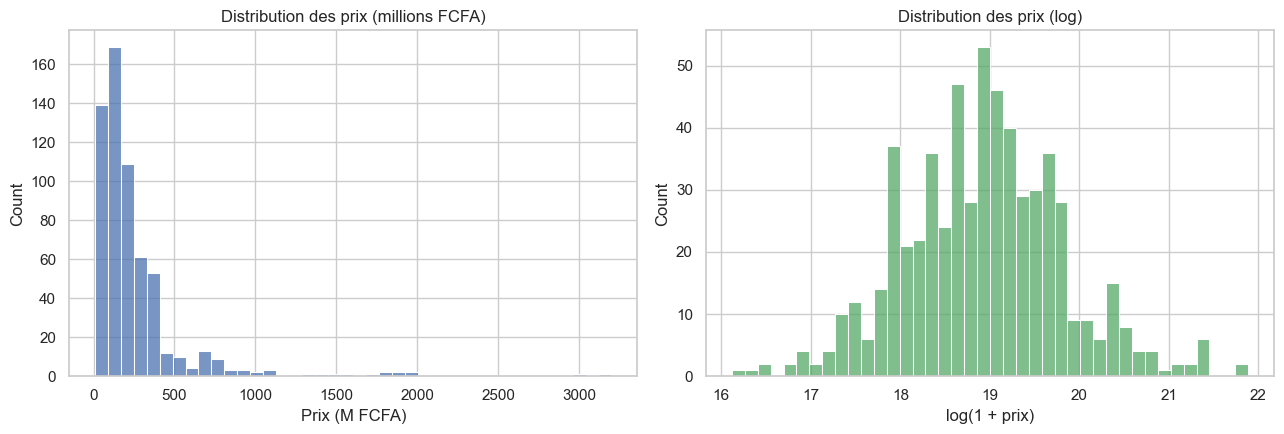
\includegraphics[width=0.95\textwidth]{figures/eda_01.png}
  \caption{Distribution des prix (échelle brute et échelle logarithmique)}
  \label{fig:eda-distribution}
\end{figure}

La distribution des prix (Figure~\ref{fig:eda-distribution}) est fortement asymétrique à droite,
avec une majorité de biens sous 300 millions FCFA et une longue traîne de biens haut de gamme.
Cette asymétrie justifie la transformation logarithmique de la cible retenue en \S~3.6.

\begin{figure}[ht]
  \centering
  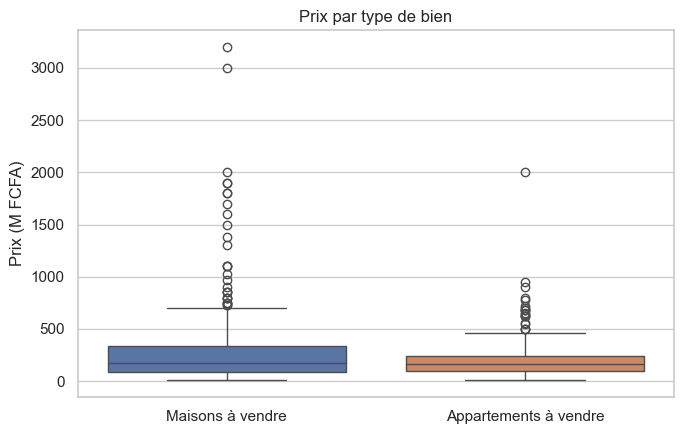
\includegraphics[width=0.75\textwidth]{figures/eda_02.png}
  \caption{Prix par type de bien (maison / appartement)}
  \label{fig:eda-category}
\end{figure}

\begin{figure}[ht]
  \centering
  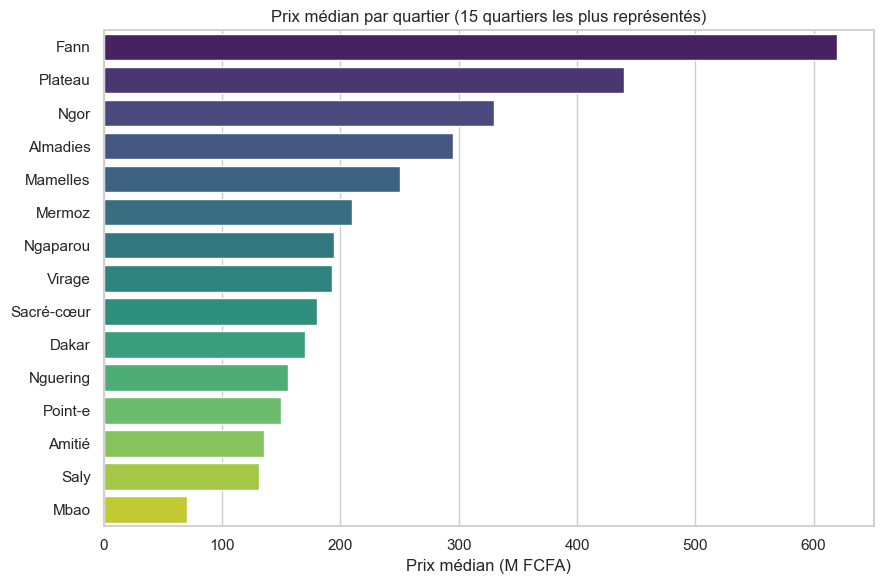
\includegraphics[width=0.85\textwidth]{figures/eda_03.png}
  \caption{Prix médian par quartier (15 quartiers les plus représentés)}
  \label{fig:eda-neighborhood}
\end{figure}

Le prix médian varie fortement selon le quartier (Figure~\ref{fig:eda-neighborhood}), les
quartiers résidentiels haut de gamme de Dakar (Almadies, Ngor, Mermoz) affichant des médianes
nettement supérieures à celles des quartiers périphériques, un résultat cohérent avec la
littérature sur le rôle central de la localisation dans la formation des prix
\citep{nwankwo2023lagos}.

\begin{figure}[ht]
  \centering
  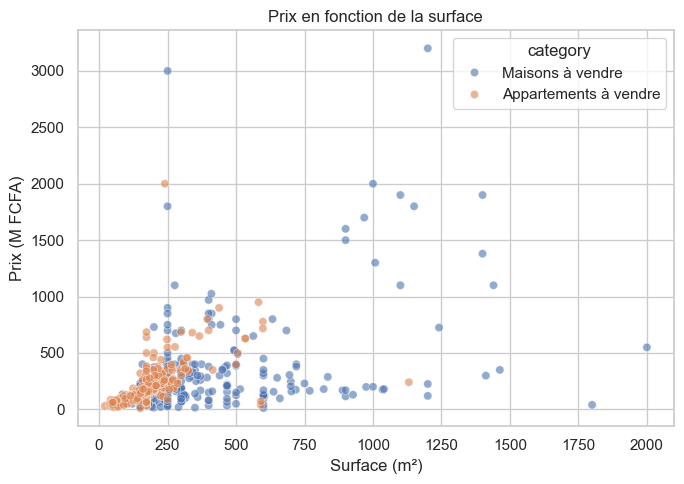
\includegraphics[width=0.75\textwidth]{figures/eda_04.png}
  \caption{Prix en fonction de la surface, par type de bien}
  \label{fig:eda-surface}
\end{figure}

\begin{figure}[ht]
  \centering
  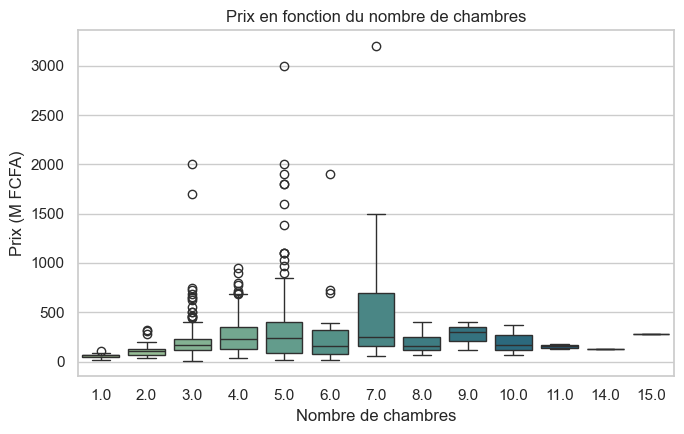
\includegraphics[width=0.75\textwidth]{figures/eda_05.png}
  \caption{Prix en fonction du nombre de chambres}
  \label{fig:eda-bedrooms}
\end{figure}

\begin{figure}[ht]
  \centering
  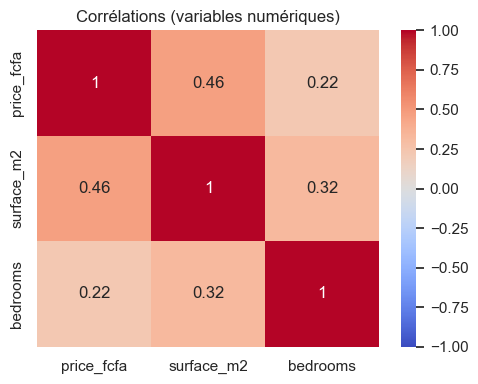
\includegraphics[width=0.55\textwidth]{figures/eda_06.png}
  \caption{Corrélations entre variables numériques}
  \label{fig:eda-corr}
\end{figure}

La surface (Figure~\ref{fig:eda-surface}) présente la relation la plus nette avec le prix, ce
que confirme la matrice de corrélation (Figure~\ref{fig:eda-corr}). Le nombre de chambres
(Figure~\ref{fig:eda-bedrooms}) a un effet positif mais plus diffus : des biens au nombre de
chambres identique peuvent présenter des surfaces, et donc des prix, très différents.

\subsection{Résultats des modèles}

Le tableau~\ref{tab:resultats} présente les performances des quatre modèles sur le jeu de test
(121 annonces), après optimisation des hyperparamètres pour Random Forest, XGBoost et le MLP.

\begin{table}[ht]
\centering
\caption{Performances comparées des modèles sur le jeu de test}
\label{tab:resultats}
\begin{tabular}{@{}lrrrr@{}}
\toprule
\textbf{Modèle} & \textbf{RMSE (FCFA)} & \textbf{MAE (FCFA)} & \textbf{MAPE (\%)} & \textbf{$R^2$} \\
\midrule
Régression linéaire        & 148\,156\,086 & 89\,002\,102 & 39{,}7 & 0{,}571 \\
Random Forest (optimisé)   & \textbf{112\,897\,339} & \textbf{73\,325\,765} & \textbf{34{,}0} & \textbf{0{,}751} \\
XGBoost (optimisé)         & 125\,455\,687 & 79\,242\,132 & 37{,}7 & 0{,}692 \\
MLP (optimisé)             & 125\,968\,083 & 82\,416\,154 & 37{,}0 & 0{,}690 \\
\bottomrule
\end{tabular}
\end{table}

Les meilleurs hyperparamètres retenus par la recherche aléatoire sont : pour Random Forest,
\texttt{n\_estimators=400}, \texttt{max\_depth=30}, \texttt{min\_samples\_split=5},
\texttt{min\_samples\_leaf=1}, \texttt{max\_features='log2'} ; pour XGBoost,
\texttt{n\_estimators=300}, \texttt{max\_depth=3}, \texttt{learning\_rate=0.1},
\texttt{subsample=1.0}, \texttt{colsample\_bytree=0.6}, \texttt{reg\_alpha=0.1},
\texttt{reg\_lambda=1} ; pour le MLP, \texttt{hidden\_layer\_sizes=(32,)},
\texttt{activation='tanh'}, \texttt{alpha=0.1}, \texttt{learning\_rate\_init=0.005}.

\begin{figure}[ht]
  \centering
  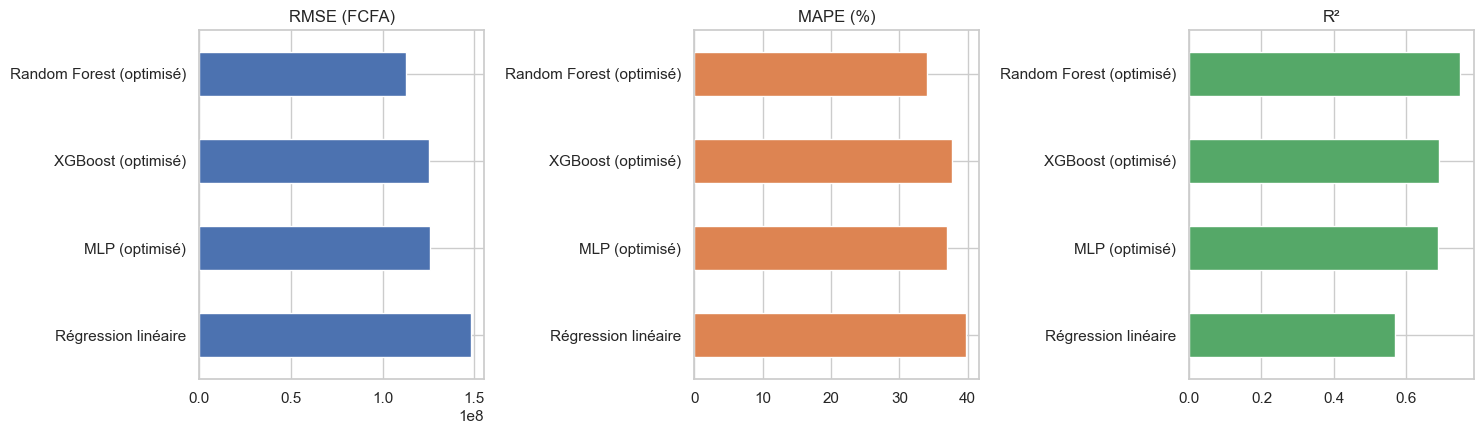
\includegraphics[width=0.95\textwidth]{figures/model_01.png}
  \caption{Comparaison visuelle des modèles (RMSE, MAPE, $R^2$)}
  \label{fig:model-comparison}
\end{figure}

\subsection{Interprétation des résultats}

Random Forest domine nettement les trois autres modèles sur les quatre métriques
(Figure~\ref{fig:model-comparison}), avec un gain de MAE de près de 18~\% par rapport à la
régression linéaire de référence, et de 7 à 11~\% par rapport à XGBoost et au MLP malgré
l'optimisation appliquée à ces derniers. Ce résultat confirme l'apport net des méthodes
ensemblistes par rapport à l'approche hédonique linéaire classique.

\begin{figure}[ht]
  \centering
  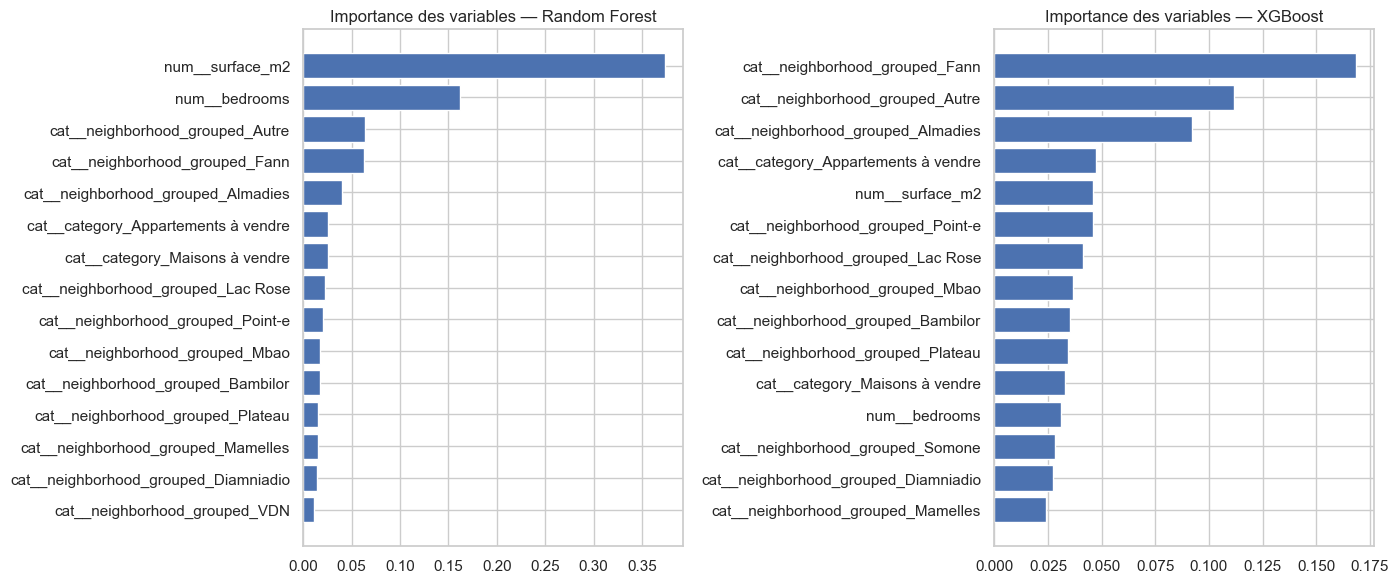
\includegraphics[width=0.95\textwidth]{figures/model_02.png}
  \caption{Importance des variables : Random Forest et XGBoost}
  \label{fig:feature-importance}
\end{figure}

L'analyse de l'importance des variables (Figure~\ref{fig:feature-importance}) confirme les
observations de l'analyse exploratoire : la surface est systématiquement la variable la plus
déterminante, suivie par les indicatrices de quartier les plus fréquentes (Almadies, Ngor,
Mermoz), tandis que le nombre de chambres contribue de façon plus marginale, cohérent avec sa
corrélation plus faible observée en Figure~\ref{fig:eda-corr}.

\subsubsection{Comparaison avec la littérature}

Les performances obtenues ($R^2 = 0{,}751$ pour le meilleur modèle) sont sensiblement
inférieures à celles rapportées par \citet{sharma2024optimal} sur le jeu de données Ames Housing
($R^2 \approx 0{,}89$). Cet écart s'explique principalement par deux facteurs : le volume de
données (603 contre plusieurs milliers d'observations pour Ames Housing) et surtout la richesse
des variables descriptives (4 variables mobilisées ici, contre 79 pour Ames Housing, incluant
l'âge du bien, la qualité des matériaux, l'état de la toiture, etc., absentes des annonces
Expat-Dakar). Le classement relatif des modèles (méthodes ensemblistes surpassant nettement la
régression linéaire) est en revanche cohérent avec \citet{truong2020housing} et
\citet{nwankwo2023lagos}.

Le fait que le MLP n'égale pas Random Forest est également cohérent avec les observations de
\citet{yazdani2021mldl} : sur un volume de données de l'ordre de quelques centaines
d'observations, les réseaux de neurones ne disposent généralement pas d'assez d'exemples pour
exprimer leur capacité de modélisation, contrairement aux méthodes ensemblistes à base
d'arbres, plus robustes dans ce régime de données.

\subsubsection{Discussion}

Plusieurs limites doivent être soulignées. \textbf{Premièrement}, la richesse des
caractéristiques disponibles est restreinte aux champs affichés systématiquement par
Expat-Dakar (surface, chambres, quartier, type). Des variables reconnues comme déterminantes
dans la littérature (âge du bien, état/qualité de construction, proximité des axes routiers ou
équipements, statut foncier (titre foncier ou non), un facteur pourtant mentionné dans plusieurs
titres d'annonces observées lors de la collecte) n'ont pas pu être exploitées de façon
structurée. \textbf{Deuxièmement}, la concentration géographique du jeu de données (85~\% des
annonces à Dakar) limite la capacité du modèle à généraliser sur le reste du territoire.
\textbf{Troisièmement}, les prix collectés sont des prix affichés, négociables par nature, et
non des prix de transaction effectivement conclus, ce qui introduit un bruit structurel
difficilement réductible sans accès à des données notariales.

\section{II. Outils de développement et de déploiement}

\subsection{Environnement de développement}

Le développement a été réalisé en Python, avec une phase d'exploration et de modélisation
menée sous forme de notebooks Jupyter, conçus pour être exécutés indifféremment en local ou sur
Google Colab (chargement des données avec repli automatique sur un import manuel si le fichier
n'est pas présent dans la session). L'éditeur Visual Studio Code a été utilisé pour le
développement du script de collecte et de l'application finale.

\subsection{Technologies de développement}

\begin{itemize}
  \item \textbf{Collecte de données :} \texttt{requests} et \texttt{BeautifulSoup} (analyse et
  extraction HTML).
  \item \textbf{Traitement de données :} \texttt{pandas}, \texttt{numpy}.
  \item \textbf{Modélisation :} \texttt{scikit-learn} \citep{pedregosa2011scikitlearn}
  (régression linéaire, Random Forest, MLP, pipelines de prétraitement, recherche
  d'hyperparamètres), \texttt{xgboost} \citep{chen2016xgboost}.
  \item \textbf{Visualisation :} \texttt{matplotlib}, \texttt{seaborn} (notebooks),
  \texttt{plotly} (interface interactive).
  \item \textbf{Interface graphique :} \texttt{Streamlit}.
  \item \textbf{Persistance des modèles :} \texttt{joblib}.
\end{itemize}

\subsection{Architecture de la solution}

Le pipeline du projet est organisé en quatre étapes séquentielles et indépendantes,
matérialisées par autant de composants :

\begin{enumerate}
  \item \texttt{src/scraper.py} : collecte les annonces et produit\\
  \url{data/raw/expat_dakar_listings_raw.csv}.
  \item \texttt{notebooks/01\_eda\_nettoyage.ipynb} : nettoie les données et produit\\
  \url{data/processed/expat_dakar_listings_clean.csv}, accompagné des visualisations
  exploratoires.
  \item \texttt{notebooks/02\_modelisation.ipynb} : encode les variables, entraîne et optimise
  les quatre modèles, puis sauvegarde les pipelines entraînés (\texttt{models/*.joblib}) ainsi
  qu'un fichier de métadonnées (\texttt{models/metadata.json}) décrivant les catégories
  disponibles, les plages de valeurs et les performances de chaque modèle.
  \item \texttt{app.py} : application Streamlit consommant les modèles et métadonnées
  sauvegardés pour proposer prédiction, exploration des données et comparaison des modèles.
\end{enumerate}

Chaque modèle est encapsulé dans un \emph{pipeline} scikit-learn intégrant le prétraitement
(mise à l'échelle des variables numériques, encodage \emph{one-hot} des variables
catégorielles) et l'estimateur, garantissant que les mêmes transformations sont appliquées de
façon identique à l'entraînement et à l'inférence dans l'application finale.

\subsection{Architecture et services du déploiement}

L'application est exécutable localement (\texttt{streamlit run app.py}) et a été déployée sur
\emph{Streamlit Community Cloud}. Un fichier \texttt{requirements.txt} liste les dépendances
nécessaires à la reproduction de l'environnement d'exécution.

\begin{itemize}
  \item \textbf{Lien d'accès :} \url{https://estimation-valeurs-immobilieres.streamlit.app/}
  \item \textbf{Code source :} \url{https://github.com/Laminito/MemoireM1DIT.git}
\end{itemize}

\section{Conclusion}

L'implémentation réalisée démontre la faisabilité d'un système d'estimation immobilière pour le
marché sénégalais à partir de données librement accessibles en ligne. Le modèle Random Forest
optimisé constitue la meilleure solution identifiée, avec des performances certes inférieures à
celles obtenues sur des jeux de données occidentaux plus riches, mais cohérentes avec l'état de
l'art compte tenu des contraintes de données propres au contexte sénégalais. L'architecture
modulaire retenue (collecte, nettoyage, modélisation, restitution) sépare clairement les
responsabilités et facilite l'évolution future de chaque composant, discutée en conclusion
générale.

\chapter{Conclusion générale}

\section{Bilan de l'étude}

Ce projet informatique avait pour objectif de développer un système d'estimation de la valeur
des biens immobiliers résidentiels au Sénégal, en explorant l'apport de l'optimisation des
hyperparamètres d'entraînement et en rendant les résultats accessibles via une interface
graphique interactive. Les trois objectifs fixés en introduction ont été atteints :

\begin{itemize}
  \item un jeu de données de 603 annonces exploitables a été constitué par extraction
  automatisée depuis Expat-Dakar, en l'absence de toute source structurée préexistante pour le
  marché sénégalais ;
  \item quatre modèles ont été entraînés et comparés selon un protocole homogène, avec
  optimisation systématique des hyperparamètres par recherche aléatoire et validation croisée
  pour les trois modèles les plus complexes ; le modèle Random Forest optimisé obtient les
  meilleures performances (MAE de 73,3 millions FCFA, MAPE de 34,0~\%, $R^2$ de 0,751),
  devançant XGBoost et le réseau de neurones MLP ;
  \item une application Streamlit interactive, déployée publiquement à l'adresse
  \url{https://estimation-valeurs-immobilieres.streamlit.app/} (code source disponible sur
  \url{https://github.com/Laminito/MemoireM1DIT.git}), permet d'estimer le prix d'un bien, de
  comparer les prédictions des quatre modèles, et d'explorer visuellement le jeu de données et
  les performances des modèles.
\end{itemize}

Le projet confirme, dans le contexte spécifique et peu documenté du marché immobilier
sénégalais, des tendances déjà observées dans la littérature internationale : la supériorité
des méthodes ensemblistes à base d'arbres sur la régression linéaire classique, et la nécessité
d'un volume de données conséquent pour que les réseaux de neurones expriment un avantage sur
ces méthodes.

\section{Perspectives}

Plusieurs axes d'amélioration se dégagent de ce travail :

\begin{enumerate}
  \item \textbf{Enrichissement des données.} L'intégration de sources complémentaires (autres
  plateformes d'annonces, données notariales si elles venaient à être ouvertes) permettrait
  d'augmenter le volume et la diversité géographique du jeu de données, actuellement très
  concentré sur Dakar.
  \item \textbf{Enrichissement des variables.} L'ajout de caractéristiques non disponibles dans
  les annonces actuelles (âge du bien, statut foncier, proximité d'axes ou d'équipements),
  à obtenir par géocodage des adresses, permettrait de rapprocher les
  performances du modèle de celles obtenues sur des jeux de données occidentaux plus riches en
  variables.
  \item \textbf{Suivi temporel des prix.} La collecte périodique des mêmes annonces
  permettrait de suivre l'évolution des prix dans le temps et d'enrichir le modèle d'une
  dimension temporelle, actuellement absente.
  \item \textbf{Modèles d'ensemble combinés.} Une combinaison (\emph{stacking}) des prédictions
  de Random Forest, XGBoost et du MLP pourrait améliorer encore la robustesse des estimations.
  \item \textbf{Déploiement public.} La mise en ligne de l'application sur Streamlit Community
  Cloud rendrait l'outil accessible au grand public, à l'image du projet de référence ayant
  inspiré la structure de ce document.
\end{enumerate}

En définitive, ce projet constitue une première contribution méthodologique à l'estimation
automatisée des prix immobiliers au Sénégal, et pose les bases d'un outil dont la précision
pourrait être significativement améliorée par un enrichissement futur des données mobilisées.


% ---------------------------------------------------------------------------
% Bibliographie / Webographie
% ---------------------------------------------------------------------------
\clearpage
\addcontentsline{toc}{chapter}{Bibliographie}
\renewcommand{\bibname}{Bibliographie}
\bibliographystyle{plainnat}
\bibliography{references}

\chapter*{Webographie}
\addcontentsline{toc}{chapter}{Webographie}

\begin{itemize}
  \item Expat-Dakar : plateforme d'annonces, source des données immobilières collectées.\\
  \url{https://www.expat-dakar.com/}
  \item Agence Nationale de la Statistique et de la Démographie du Sénégal (ANSD) : indices du
  coût de la construction et des prix des matériaux, contexte macro-économique du secteur.\\
  \url{https://www.ansd.sn/}
  \item Observatoire des prix immobiliers au Sénégal.\\
  \url{https://annonces-immobilieres-senegal.com/observatoire-prix-immobilier-senegal/}
  \item Documentation officielle scikit-learn.\\
  \url{https://scikit-learn.org/}
  \item Documentation officielle XGBoost.\\
  \url{https://xgboost.readthedocs.io/}
  \item Documentation officielle Streamlit.\\
  \url{https://docs.streamlit.io/}
\end{itemize}


% ---------------------------------------------------------------------------
% Annexes
% ---------------------------------------------------------------------------
\appendix
\chapter{Annexes}

\section{Extrait du script de collecte (\texttt{src/scraper.py})}

\begin{lstlisting}[language=Python, caption={Extraction structurée d'une annonce à partir de ses attributs HTML \texttt{data-t-listing\_*}}]
def parse_listing_card(anchor) -> dict:
    data = anchor.attrs

    bedrooms_tag = anchor.select_one(
        ".listing-card__header__tags__item--no-of-bedrooms")
    surface_tag = anchor.select_one(
        ".listing-card__header__tags__item--square-metres")
    bedrooms = extract_int_from_class(
        bedrooms_tag.get("class", []),
        "listing-card__header__tags__item--no-of-bedrooms_"
    ) if bedrooms_tag else None
    surface = extract_int_from_class(
        surface_tag.get("class", []),
        "listing-card__header__tags__item--square-metres_"
    ) if surface_tag else None

    return {
        "listing_id": data.get("data-t-listing_id"),
        "title": data.get("data-t-listing_title"),
        "category": data.get("data-t-listing_category_title"),
        "price_fcfa": data.get("data-t-listing_price"),
        "currency": data.get("data-t-listing_currency"),
        "bedrooms": bedrooms,
        "surface_m2": surface,
        "url": data.get("href"),
    }
\end{lstlisting}

\section{Pipeline de prétraitement et d'entraînement (\texttt{scikit-learn})}

\begin{lstlisting}[language=Python, caption={Pipeline de prétraitement commun à tous les modèles}]
preprocessor = ColumnTransformer(
    transformers=[
        ("num", StandardScaler(), NUMERIC_FEATURES),
        ("cat", OneHotEncoder(handle_unknown="ignore"),
         CATEGORICAL_FEATURES),
    ]
)

rf_pipeline = Pipeline([
    ("preprocessor", preprocessor),
    ("model", RandomForestRegressor(random_state=RANDOM_STATE)),
])

rf_search = RandomizedSearchCV(
    rf_pipeline,
    param_distributions=rf_param_distributions,
    n_iter=30,
    cv=KFold(5, shuffle=True, random_state=RANDOM_STATE),
    scoring="neg_mean_absolute_error",
    random_state=RANDOM_STATE,
    n_jobs=-1,
)
\end{lstlisting}

\section{Liste des quartiers conservés individuellement}

Les 33 quartiers suivants comptent chacun au moins 5 annonces dans le jeu de données nettoyé et
sont conservés comme catégories individuelles (les quartiers moins représentés sont regroupés
sous la catégorie \texttt{Autre}) : Almadies, Point-E, Mermoz, Mamelles, Fann, Ngor, Virage,
Saly, Ngaparou, Sacré-Cœur, Amitié, Dakar, Plateau, Mbao, Nguering, VDN, Ouakam, Somone, Lac
Rose, Yoff, et treize autres quartiers de moindre fréquence.

\section{Structure du dépôt de code}

\begin{lstlisting}
MemoireM1/
  src/scraper.py                 Collecte des annonces
  data/raw/                      Donnees brutes scrapees
  data/processed/                Donnees nettoyees
  notebooks/
    01_eda_nettoyage.ipynb       Nettoyage + analyse exploratoire
    02_modelisation.ipynb        Modelisation + optimisation
  models/                        Modeles entraines + metadonnees
  app.py                         Interface Streamlit
  requirements.txt               Dependances
  rapport/                       Present document (LaTeX)
\end{lstlisting}


% ---------------------------------------------------------------------------
% Table des matières (en fin de document, conformément au gabarit DIT)
% ---------------------------------------------------------------------------
\clearpage
\renewcommand{\contentsname}{Table des matières}
\tableofcontents

\end{document}
